\section{Theorie}
\label{sec:Theorie}

%In knapper Form sind die physikalischen Grundlagen des Versuches, des Messverfahrens, sowie sämtliche %für die Auswertung erforderlichen Gleichungen darzustellen. (Keine Herleitung)

%(eventuell die Aufgaben)

%Der Versuchsaufbau: Beschreibung des Versuchs und der Funktionsweise (mit Skizze/Bild/Foto)

Ein elektrischer Schwingkreis ist eine Schaltung bestehend aus einem Widerstand $R$, einer Spule $L$ und einem Kondensator $C$. 
Schwingkreis heißt diese Schaltung, weil sie beschrieben werden kann wie ein harmonischer Oszillator, in dem die Spannungsamplitude und die Stromamplitude gegenphasig hin und her schwingen.
Gekoppelt werden zwei Schwingkreise über einen zusätzlichen Kondensator $C_k$. (siehe \autoref{fig:schaltung_1})
Eine gleiche Resonanzfrequenz der beiden Schwingkreise muss vorausgesetzt sein. 
Dies kann man analog ansehen wie zwei identische Fadenpendel, welche mit einer Feder gekoppelt sind.

\begin{figure}
    \label{fig:schaltung_1}
    \centering
    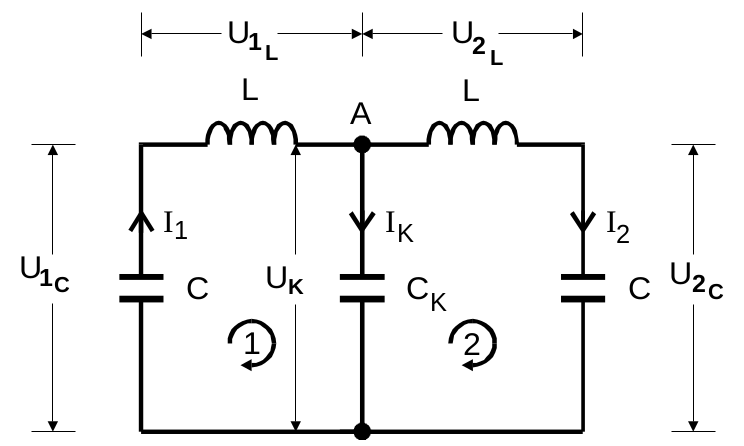
\includegraphics[width=\textwidth/3]{images/schaltung_1.png}
    \caption{Schaltbild der hier beschriebenen gekoppelten Schwingkreisen. \cite{V355}}
\end{figure}
